\section{Genkidama}

	\subsection{Introducción}
    El problema a resolver trata de,dado un T(luego explicaremos), intentar "matar"  de manera optima(menor cantidad de disparos) enemigos(puntos en un plano $\mathbb{N}^{2}$) que siguen un invariante particular:\\
-los puntos  $(x_i,y_i)\textrm{cumplen} \quad i>j \Rightarrow x_i > x_j \wedge y_i < y_j$\\
Mas informalmente, se ordenan de derecha a izquierda y de abajo hacia arriba.
\\
\\
Donde el termino "matar" se define de la siguiente manera:
$p_i=(x_i,y_i) \textrm{ mata a } p_j=(x_j,y_j) \textrm{ si y solo si: }$
$x_i+T \geq x_j \wedge y_i+T \geq y_j$
\\
\\
Es inmediato encontrar un algoritmo cuadratico que resuelva este problema, el dasafio entonces esta en realizar uno de complejidad lineal.
    \subsection{Desarrollo}


    		\subsubsection*{Descripción}
		 
	   	Como el objetivo es matar a todos realizando la menor cantidad de disparos, lo que vamos a hacer es buscar cual es el último guerrero a quien se le pueda disparar desde el cual siga matando al primero de la lista. Allí será donde se disparará la primer Genkidama. Una vez realizado el disparo se buscará cual es el primer soldado que sobrevivió al ataque y se reiniciará el problema tomando a ese guerrero como el nuevo primero. Éste proceso se repetirá hasta que no queden mas guerreros enemigos vivos. \\

		
		MataAl:
		Ésta función recibe por parámetro el valor del $T$,  un vector de puntos en el plano que representa los guerreros enemigos y dos enteros que representan posiciones en el vector.  El resultado es un booleano que indica si disparándole una Genkidama al enemigo ubicado en la posición $i$ mata al de la posición $j$ también.\\

		\begin{algoritmo}{MataAl}{\In{i}{int}, \In{j}{int}, \In{N}{int}, \In{T}{int}, \Inout{enemigos}{vector(pair(int,int))} }{bool}
		  \eIf{cuando disparo al que esta en la posición $i$ mata al que esta en la posición $j$}{
    		devolver true \;
  				}{
    		devolver false \;
  			}

		\end{algoritmo}
		
		MasLejanoQueMata:
		Ésta función recibe por parámetro el valor del $T$, un vector de puntos en el plano que representa los guerreros enemigos y un entero que indica la posición de un soldado en el vector.
		La función devuelve la posición del ultimo guerrero que muere en caso de dispararle al que ocupa la posición pasada por parámetro.\\

		\begin{algoritmo}{masLejanoQueMata}{\In{aEsteLeDisparo}{int}, \In{N}{int}, \Inout{enemigos}{vector(pair(int,int))}}{int}
			j = i + 1;\;
			\While{si le disparo al que esta en la posición $i$ mata al que está en la posición $j$}{
    		j++ \;
  			}
  			devolver j - 1; // Cuando sale del ciclo $j$ el la posición del primer guerrero que queda vivo en caso de dispararle al que ocupa la posición $i$ entonces hay que restarle uno para devolver la posición del último que muere.\;
		\end{algoritmo}

		
		MasLejanoQueMataAl:
		Ésta función recibe por parámetro el valor del $T$,  un vector de puntos en el plano que representa los guerreros enemigos y un entero que indica la posición de un soldado en el vector.
		La función devuelve la posición del ultimo guerrero al cual puedo disarale pero que siga matando al enemigo que ocupa la posicion pasada por parametro.\\ 

	\begin{algoritmo}{masLejanoQueMataAl}{\In{i}{int}, \In{N}{int}, \In{T}{int}, \Inout{enemigos}{vector(pair(int,int))}}{int}
		j = i + 1 \;
		\While{si le disparo al que esta en la posición $j$ sigue matando al que esta en la posición $i$}{
    		j++ \;
  		}
  		j = j - 1;\; //cuando sale del ciclo $j$ es la posición del primer guerrero al que hay que dispararle y que no mate al $i$. Como tiene que matarlo se retrocede uno. 

	\end{algoritmo} \;

		
		Genkidama:
		Ésta función recibe por parámetro el valor del $T$,  un vector de puntos en el plano que representa los guerreros enemigos y su longitud, y un puntero a una lista de enteros donde se guardarán los guerreros a los cuales será necesario lanzar genkidamas. Devolverá tambien la cantidad de disparos realizados. \\

	\begin{algoritmo}{genkidama}{\In{N}{int}, \In{T}{int}, \In{enemigos}{vector(pair(int,int))}, \Inout{DisparosEfectuados}{list(int)}}{int}

		int cantGenkidamas=0;
  		int i=0;
  		\While{$i < n$}{
    		int aEsteLeDisparo=masLejanoQueMataAl(i,N,T,enemigos);//busco el mas lejano que mate al primero de los que quedan vivos \;
    		i = masLejanoQueMata(aEsteLeDisparo,N,T,enemigos) + 1;//empiezo a preguntar desde el sigiente al ultimo en morir\;
    		agregar AEsteLeDisparo a la lista de disparos efectuados;\;
    		cantGenkidamas++; \;
  		}
  		devolver cantGenkidamas; \;
	\end{algoritmo} \;
	
	    \subsubsection*{Correctitud}

    	
    	Para demostrar que este algoritmo resuelve el problema de manera eficiente utilizaremos dos lemas:
    		\subsubsection*{Lema 1}

    			Sean $v_{i}$, $v_{j}$ las coordenadas de dos guerreros enemigos. Si se lanza una Genkidama a $v_{j}$ y con la explosión de la misma también muere $v_{i}$, entonces $ \forall h \in (i,j), v_{h}$ morirá también. 

    		\subsubsection*{Demostración Lema 1}

    			Sean $v_{i}$ = ($x_{i}$, $y_{i}$), $v_{j}$ = ($x_{j}$, $y_{j}$) y $v_{h}$ = ($x_{h}$, $y_{h}$) posiciones de guerreros enemigos con $i < j < h$.
    			Sabemos que $x_{i} > x_{j}$ y $y_{i} < y_{j}$ porque las $x$ son decrecientes y las $y$ crecientes.

    			Quiero ver que $x_{j} + T \geqslant x_{h}$ y que $y_{j} + T > y_{h}$.

    			Veamos primero que $x_{j} + T \geqslant x_{h}$:

    			Sabemos que $x_{j} + T \geqslant x_{i}$ porque disparando en $x_{j}$ muere $x_{i}$ y además $x_{i} > x_{h}$ entonces juntando éstas dos propiedades podemos asegurar que $x_{j} + T > x_{h}$.

    			Ahora veamos que $y_{j} + T > y_{h}$:

    			Sabemos que $y_{j} > y_{h}$ y como $T > 0$ entonces $y_{j} + T > y_{h}$.

    			Entonces queda demostrado que todos los gurreros que se encuentren entre $v_{i}$ y $v_{j}$ mueren cuando se lanza una Genkidama a $v_{j}$.

    		\subsubsection*{Lema 2}

    			Sean $j$ y $k$ posiciones de guerreros enemigos tal que disparandole al que se encuentra en la posición $j$ el elemento de mayor índice que muere es el de la posición $k$, si le disparo a $i$ (con $i < j$) no puede morir el de la posición $k+1$.


    		\subsubsection*{Demostración Lema 2}
    			Demostración por el absurdo:

    			Como disparandole al soldado de la posición $j$ mata al de la posición $k$ entonces sabemos que $x_{j} - T \leq x_{k}$.
    			Como disparandole al guerrero de la posición $j$ no mata al de la posición $k+1$ entonces $x_{j} - T > x_{k+1}$
    			También sabemos que $x_{j} < x_{i}$ porque las $x$ son decrecientes.

    			Supongamos que disparando en la posición $i$ mato al enemigo de la posición $k+1$, entonces $x_{i} - T < x_{k+1}$.
    			entonces tenemos que $x_{j} - T > x_{k+1}$ y además $x_{i} > x_{j}$. Por esto último, si restamos $T$ en ambos lados queda que $x_{i} - T > x_{j} - T$, pero sabiamos que $x_{j} - T > x_{k+1}$ entonces $x_{i} - T > x_{k+1}$ lo que es absurdo porque contradice la hipótesis. 
    			Por lo tanto $x_{i}$ no puede matar a $x_{k+1}$. \\
    			\\
    			\\


		Es fácil ver que con esta forma de resolución se mueren todos los enemigos ya que se toma el primer guerrero y se busca cual es la posición mas lejana a la cual puedo lanzar una genkidama y aun así matar al guerrero en cuestión. Por el lema 1, todos los guerreros que se encontraban entre el primero y el soldado a quien se le disparó también morirán. Luego se avanza hasta el primer enemigo que haya quedado vivo del lado derecho y se repite el mismo procedimiento partiendo del primer enemigo que sobrevivió al ataque. \\ 


		Veamos ahora que esta es la forma óptima de arrojar las Genkidamas:\\


		Como seguro en algún momento va a ser necesario matar al primero entonces vamos a matarlo tirando la Genkidama en un lugar estratégico generando que mueran la mayor cantidad de guerreros posibles junto con el enemigo en cuestión. Para ello, la manera mas eficiente de disparar la genkidama es buscar cual es el último guerrero a quien se le pueda disparar desde el cual siga matando al primero, ya que cualquier otro disparo genarará una menor o igual cantidad de muertes.\\
		Sean $i$, $j$, $k$ guerreros enemigos donde $j$ representa el último guerrero al que le puedo disparar para matar a $i$. $k$ es el último guerrero que muere cuendo lanzo la Genkidama en $j$.\\
		Por el lema 2 se sabe que si disparo en cualquier guerrero que se encuentre entre $i$ y $j$ puede pasar que mate a $k$ o no, pero nunca puede pasar que mate al soldado que se encuentra en la posición $k+1$. Entonces si disparo la Genkidama en un $x_{h}$ con $h \in (i, j)$ no mato mas guerreros de los que mataba tirándola en $x_{j}$ del lado derecho, pero si puede pasar que mate menos, por ejemplo cuando no mata al $x_{k}$.\\
		Por lo tanto ésta es una de las formas óptimas de tirar la Genkidama para matar al primer soldado enemigo.\\
		Como el algoritmo se repite cada vez que es lanzada una Genkidama tomando como guerrero nicial el último que quedo vivo, entonces debemos volver a dispararle a este de la forma mas eficiente posible. Por lo tanto el algoritmo es eficiente.  \\





    \subsection{Complejidad}
    Se cumple la complejidad pedida de $\mathcal{O}(N)$ pues,   basicamente el algoritmo consta de 3 partes:\\
    (1) La funcion que ejecuta "masLejanoQueMataAl", esta dado un indice i (que siempre sera el primero de los que aun estan vivos) dice cual es el punto  de mayor indice(digamos j) que mata a i. Esta funcion tarda $\mathcal{O}(j)$ pues son j consultas de "matasAl" y otras operaciones $\mathcal{O}(1)$ , como ya dijimos siendo j el ultimo(de indice mayor) que mata a i.\\
 Asi procedo a la parte (2) que es la funcion "masLejanoQueMata" que se le dice a quien se matara (siguiendo el nombre del punto anterior se le diria: j) y esta funcion devolvera un indice k siendo el ultimo que muere disparando a j y tardara $\mathcal{O}(k-j)$ pues recorre las posiciones entre j y k realizando operaciones $\mathcal{O}(1)$.\\
 Observamos que la complejidad de (1) y (2) en conjunto es: 
 $\mathcal{O}(j) + \mathcal{O}(k-j) =\mathcal{O}(k)  $\\
(3)Por ultimo esta secuencia de operaciones de ejecuta tantas veces como sea necesaria para muera todos los puntos, empezando desde el k de la repeticion anterior. Es decir se ejecutaran digamos $h \gets \{1..t..h\}$ iteraciones de complejidad  $\mathcal{O}(k_t)$ donde no es estrictamente importante cuanto vale cada $k_t$ pero si saber que $\sum_{t=1}^{h} k_t = n$ entonces la complejidad de ejecutar h veces este grupo de funciones de complejidad $ \mathcal{O}(k_t) $ con k como fueron descriptas previamente, sera del orden $ \mathcal{O}(\sum_{t=1}^{h} k_t)=\mathcal{O}(N) $.
    


    \subsection{Experimentación}


    	\subsubsection*{Experimento 1}\;
			En este experimento se analizará la variación del tiempo de ejecución del algoritmo cuando varía la cantidad de guerreros enemigos dejando fijo el parámetro $T$. Para ello se generarán diferentes archivos con las coordenadas de los enemigos, uno por cada tamaño de bando contrario. Las coordenadas de los soldados serán aleatorias tomando una cota como máximo valor posible para las variables x e y. Luego pasando esos archivos como parámetro de entrada al problema de genkidama, se medirán los tiempos de ejecución. \;

		\subsubsection*{Datos de entrada}\;
			Los tamaños del bando enemigo tomados fueron  desde $50$ hasta $1000$ de $50$ en $50$. \;
			El valor de $T$ utilizado fue $50$.\;
			Para generarlos se utilizó el generador.cpp que se encuentra en la carpeta exp/genkidama/exp1 y para correrlo se utilizó el exp1.sh que se encuentra en la misma carpeta. \;
			Con el fin de acercarse a los valores reales y descartar posibles falsos resultados, se ejecuta la resolución del problema para cada uno de los tamaños de equipo siete veces y se calcula el promedio de los tiempos medidos.\;

      	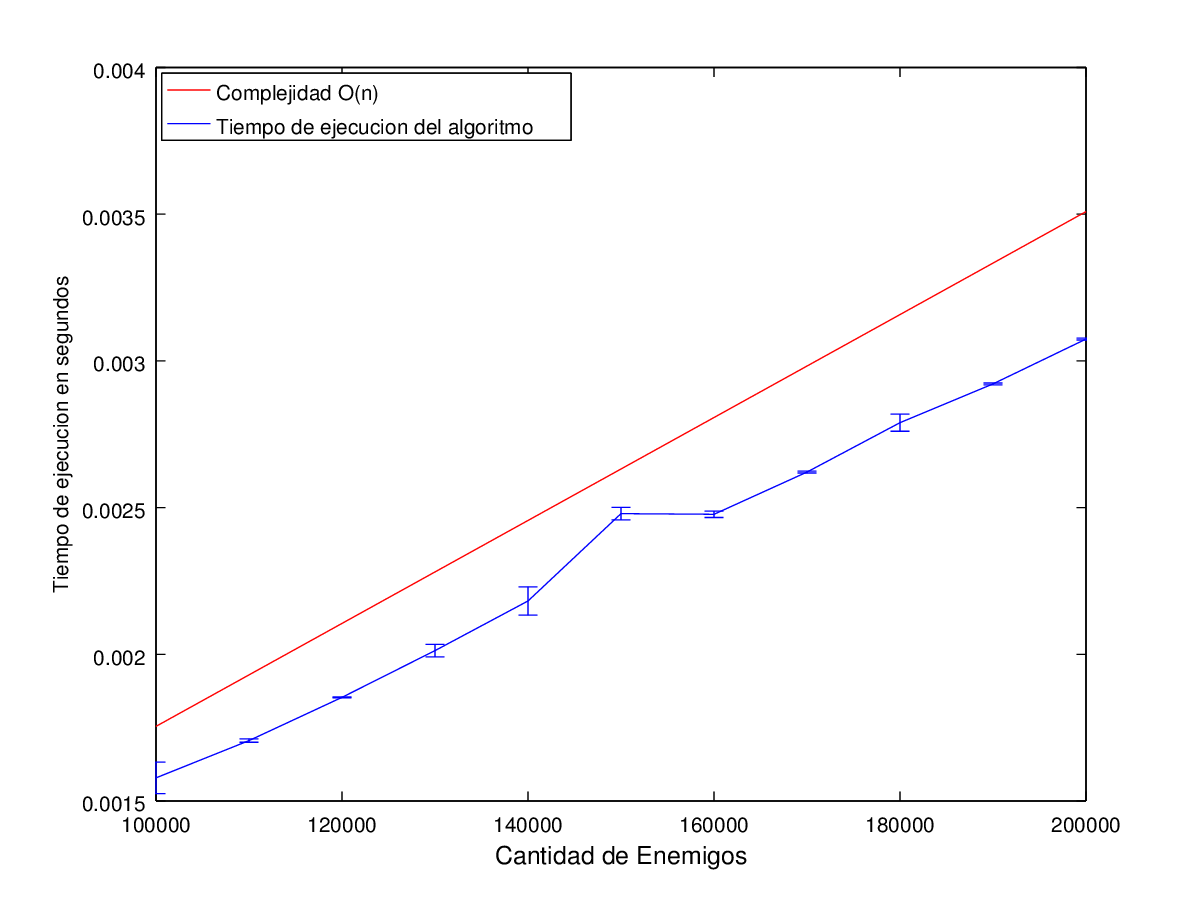
\includegraphics[height=11cm]{graficos/genkidama-exp1.png}


    	\subsubsection*{Conclusiones}
			Como se puede observar en el gráfico, el tiempo de ejecución aumenta de manera lineal con respecto a la cantidad de guerreros enemigos. Esto es así ya que el algoritmo recorre todos los puntos sin importar la distancia que haya entre ellos y la cantidad de disparos a realizar. Por ello podemos asegurar que la complejidad es de o(N).
			\\



		\subsubsection*{Experimento 2}\;
			En este experimento vamos a observar como varia el tiempo de ejecución para diferentes valores del parámetro $T$ dejando constante la cantidad de guerreros enemigos.\;


		\subsubsection*{Datos de entrada}

		
			Los valores de $T$ utilizados fueron $50$ $70$ $80$ $90$ $100$ $120$ $130$ $140$ $150$ $170$ $190$ $200$.\;
			La cantidad de guerreros en el equipo contrario utilizada fue 1000
			Para generarlos se utilizó el generador.cpp que se encuentra en la carpeta exp/genkidama/exp2 y para correrlo se utilizó el exp2.sh que se encuentra en la misma carpeta.\;
			Con el fin de acercarse a los valores reales y descartar posibles falsos resultados, se ejecuta la resolución del problema para cada uno de los valores de $T$ siete veces y se calcula el promedio de los tiempos medidos.\;
      	

      	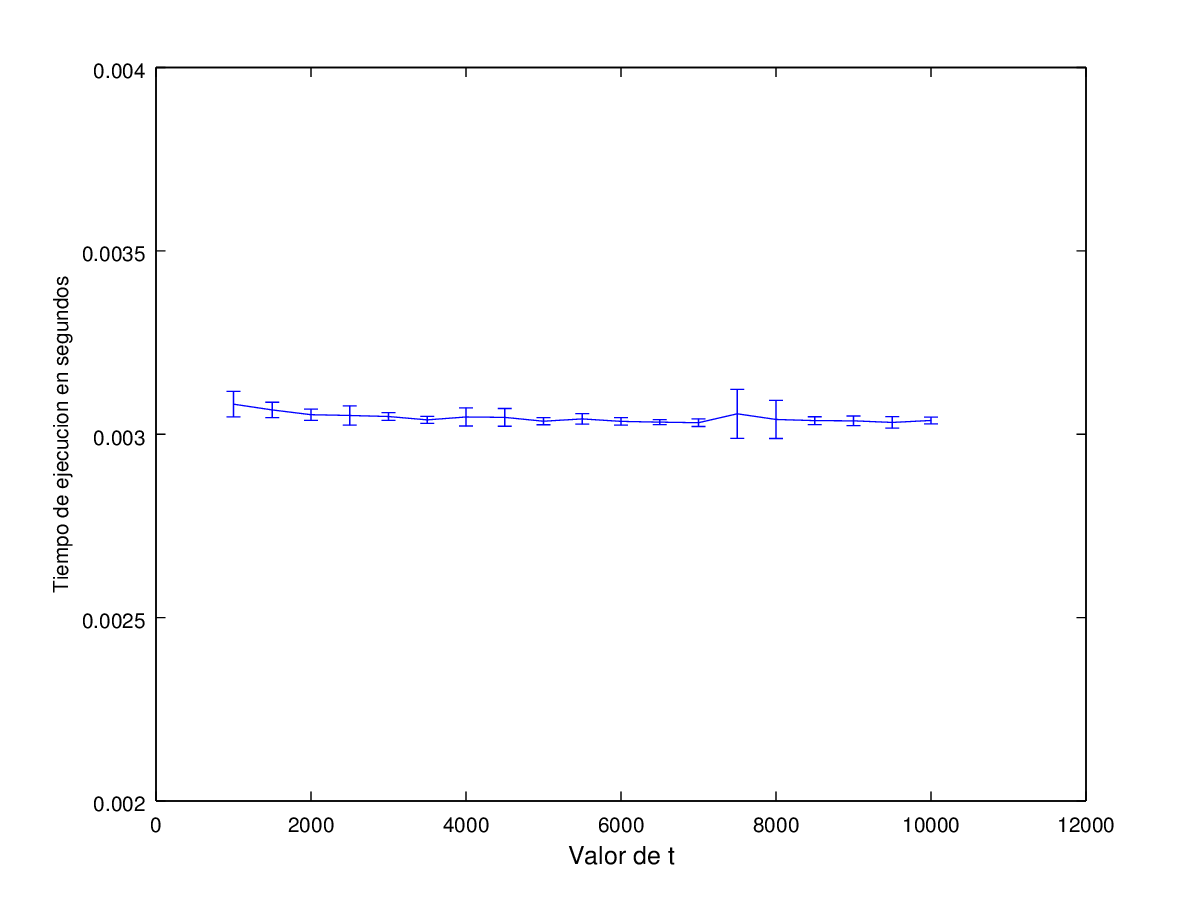
\includegraphics[height=11cm]{graficos/genkidama-exp2.png}

    	
    	\subsubsection*{Conclusiones}


			Como se puede observar,las variaciones en el tiempo de ejeucion para cada $T$ son despreciables por lo tanto se puede decir que no importa como varia el $T$, el tiempo que tarda en ejecutar el algoritmo es el mismo cuando la cantidad de puntos no varia.\;

		\;

    	\subsubsection*{Experimento 3}

			En este experimento vamos a observar como varia el tiempo de ejecución del algoritmo para casos bordes. En el primero tomaremos guerreros que se encuentren a muy poca distancia  unos de otros y en el segundo los enemigos estarán separados por grandes distancias, dejando siempre constante la cantidad de soldados. Luego mediremos los tiempos de ejecución del algoritmo genkidama para ambos casos tomando un valor de $T$ grande y luego uno chico.\;

		
		\subsubsection*{Datos de entrada}


			Los valores de $T$ utilizados fueron $4$ y $50$.
			La cantidad de guerreros en el equipo contrario utilizada fue 1000.
			En el primero las distancias eran de 2 entre soldados y en el segundo de $50$.
			Para generarlos se utilizó el generadorJuntos.cpp y el generadorSeparados.cpp  que se encuentran en la carpeta exp/genkidama/exp3.
			Para correrlo se utilizó el exp3.sh 
			Con el fin de acercarse a los valores reales y descartar posibles falsos resultados, se ejecuta la resolución del problema para cada uno de los valores de $T$ siete veces y se calcula el promedio de los tiempos medidos.\;


      	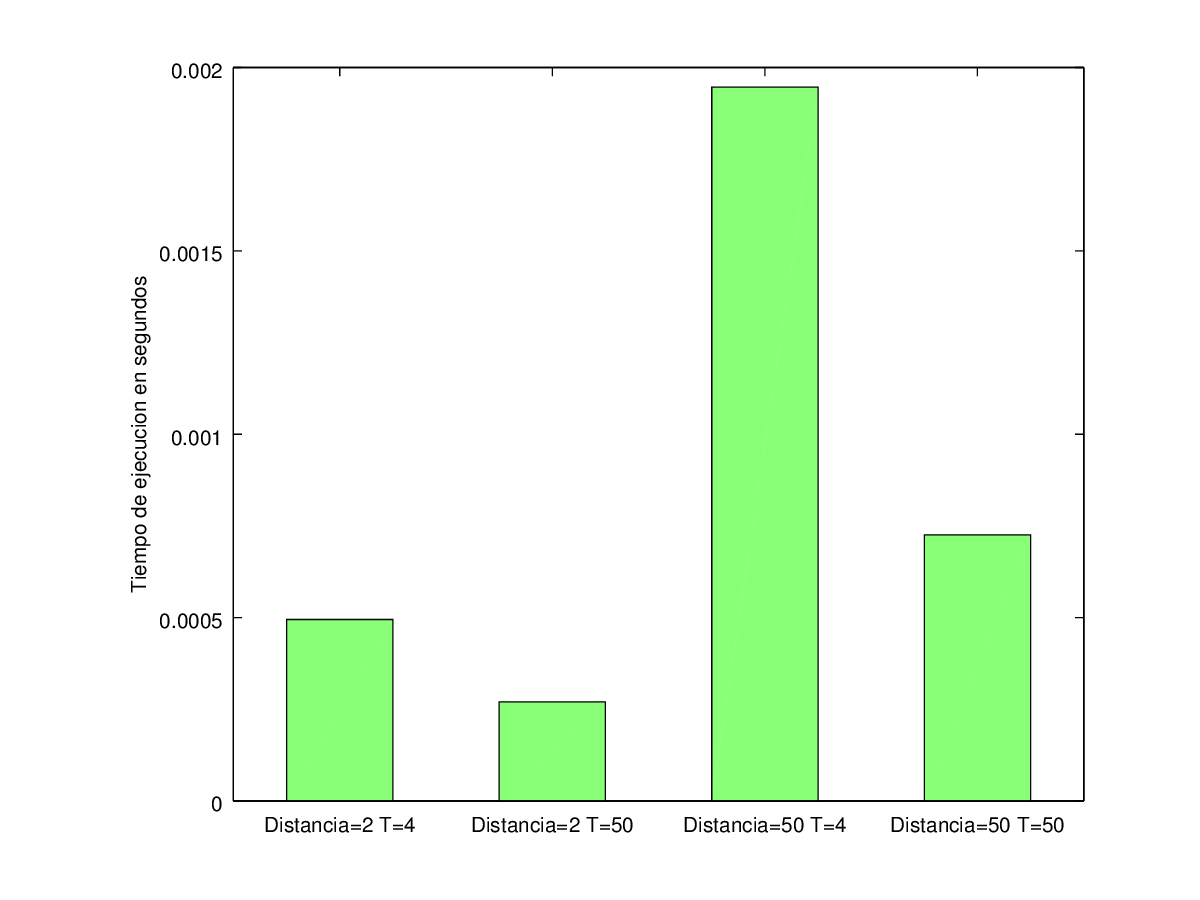
\includegraphics[height=11cm]{graficos/genkidama-exp3.png}


    	\subsubsection*{Conclusiones}\;

			Como se puede observar en el gráfico, cuando los puntos se encuentran muy distantes unos de otros y se utiliza un valor de $T$ muy chico el tiempo de ejecución es muy alto. 
			Esto se debe a que el algoritmo toma el primer guerrero y se fija cual es el ultimo al cual puede disparar si quiere matar al primero recorriendo todos los que confirmen este hecho y luego retrocediendo uno cuando le dicen que no. Luego dispara la genkidama, y avanza hasta el primer guerrero que haya sobrevivido y vuelve a comenzar. Esto se repite hasta que no queden guerreros vivos. En el caso de que todos los guerreros se encuentren a tanta distancia como para que sea necesario lanzar una genkidama por cada uno de ellos entonces el algoritmo avanzará de a uno y en cada paso avanza y retrocede uno generando así que la complejidad sea de $\mathcal{O}(2N)$. 
